\chapter{Results}
\label{chapter:results}
\gls{NCLT} dataset was used for the comparison of different filters. Functionality of each component has been tested with \gls{KITTI}, \gls{KAIST} and \gls{NCLT} datasets.



%%%%%%%%% ch start %%%%%%%

\section{Comparison of Bayesian filters}
Data from the \gls{NCLT} dataset has been used for this comparison and the results shown in the discussion have been obtained using sequence 2013.01.10.
\subsection{Translational performance}
Overall performances of all the filters are better than the raw \gls{GNSS} measurements. \gls{UKF} has given the worst estimation while \gls{PF} and \gls{ESKF} have given better results. Table \ref{table:ch:RMSErrorPosition} shows a summary of the results.
\begin{table}[h]
    \centering
    \begin{tabular}{|p{2.5cm}|p{2.5cm}|p{2.5cm}|p{2.5cm}|p{2.5cm}|} 
        \hline
            
        \textbf{Method} & \textbf{x} & \textbf{y} & \textbf{z}& \textbf{Overall} \\
        \textbf{} & \textbf{direction(m)} & \textbf{direction(m)} & \textbf{direction(m)}& \textbf{position(m)} \\
        \hline
        GPS&6.3278 &9.8746 &5.6387& 13.0133\\
        \hline
        ESKF &4.6824& 2.8655 &7.0109 &8.9044\\
        \hline
        UKF &4.7371& 2.7663 &11.2554 &12.5211
        \\
        \hline
        PF& 4.4488& 2.8587& 6.8126& 8.6242
        \\
        \hline
    \end{tabular}
\caption{Translational \gls{RMS} errors for different Bayesian filters}
\label{table:ch:RMSErrorPosition}
\end{table}

Even though \gls{PF} has given the most accurate results, as shown in figures \ref{fig:ch:errorX} to \ref{fig:ch:errorPositionOverall}, output of the filter is not smooth. Furthermore, the estimate rapidly diverges upon receiving erroneous \gls{GNSS} measurements (see figure \ref{fig:ch:errorPositionOverall}). Adding random samples or increasing the size of the particle set are alternatives for this problem. However, both of these solutions will increase the computational complexity. If both \gls{RMS} error and smoothness are considered, \gls{ESKF} gives the best solution. Z-direction has shown the worst error in all the three filters resulting a large overall positional error. This behaviour is a result of the large error in the altitude measurement, obtained by the \gls{GNSS} receiver. It can be mitigated by using an Altimeter (which is only present in the \gls{KAIST} dataset, out of the three datasets being used).

\begin{figure}[h]
    \centering
    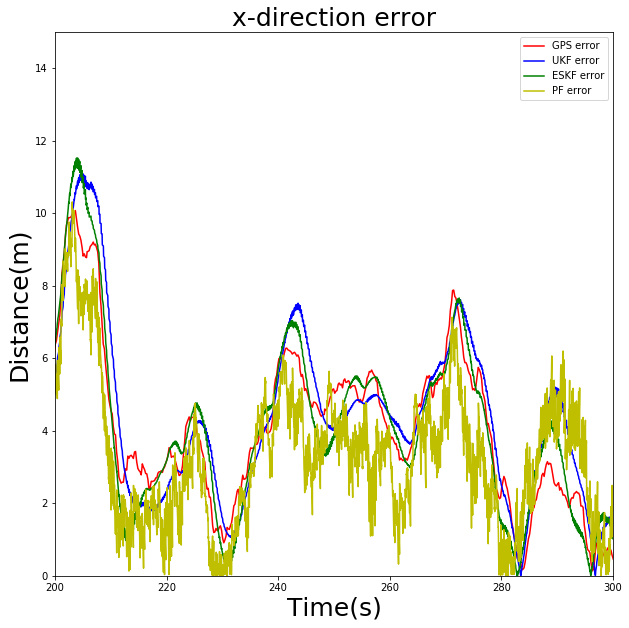
\includegraphics[width=0.7\textwidth]{figs/x_direction.png}
    \caption{Filter comparison - error in x direction}
    \label{fig:ch:errorX}
\end{figure}
\begin{figure}[h]
    \centering
    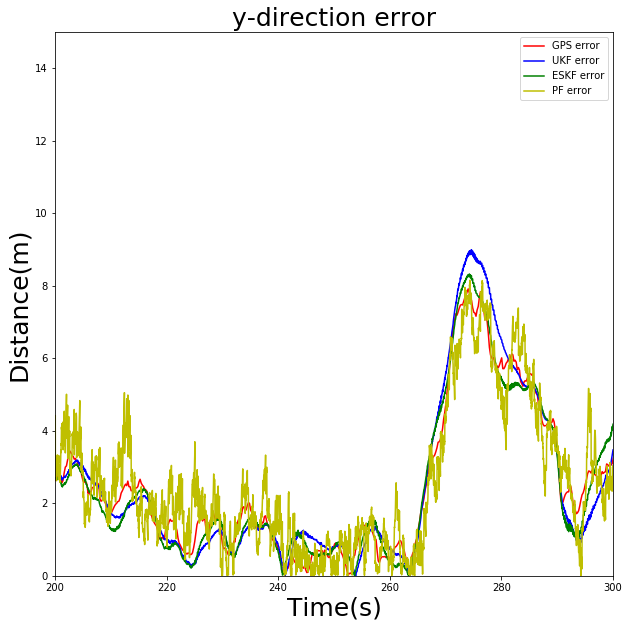
\includegraphics[width=0.7\textwidth]{figs/y_direction.png}
    \caption{Filter comparison - error in y direction}
    \label{fig:ch:errorY}
\end{figure}
\begin{figure}[h]
    \centering
    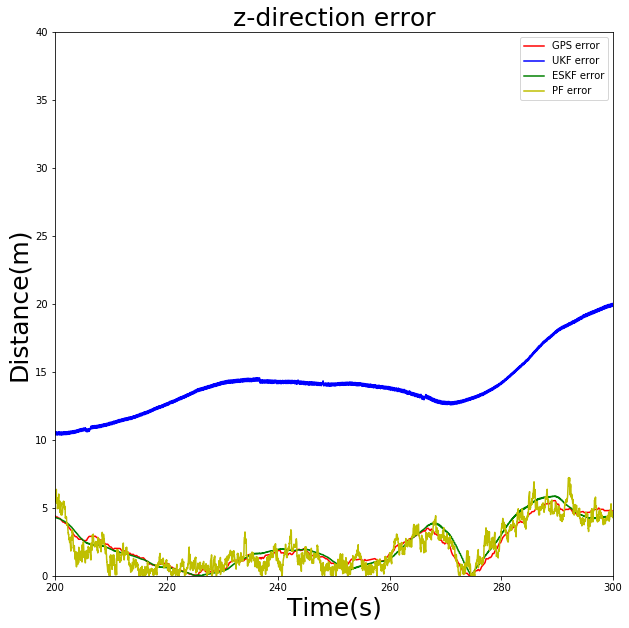
\includegraphics[width=0.7\textwidth]{figs/z_direction.png}
    \caption{Filter comparison - error in z direction}
    \label{fig:ch:errorZ}
\end{figure}
\begin{figure}[h]
    \begin{subfigure}{0.5\textwidth}
        \centering
        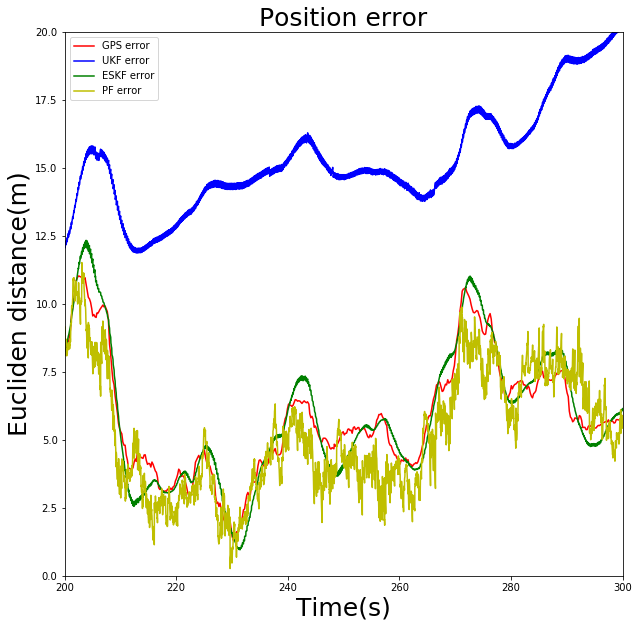
\includegraphics[width=1\textwidth]{figs/overall.png}
        \caption{Excluding the diverged \gls{PF} result}
    \end{subfigure}%
    \begin{subfigure}{0.5\textwidth}
        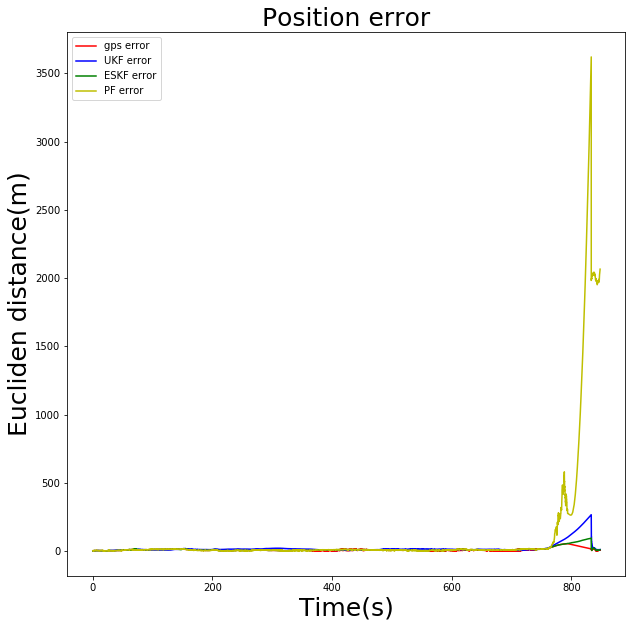
\includegraphics[width=1\textwidth]{figs/overall_diverge.png}
        \caption{Including the diverged \gls{PF} result}
    \end{subfigure}
    \caption{Filter comparison - overall translational error}
    \label{fig:ch:errorPositionOverall}
\end{figure}


\subsection{Orientation}
Raw orientation measurement obtained using the \gls{IMU} + Magnetometer is better than the estimates of all the three filters (see table \ref{table:ch:RMSErrorRotation}). This is due to the noise in the angular velocity measurement, which is confirmed from the reduction of the error when the angular measurement noise variance parameter is increased. \gls{PF} has given the worst estimation. Results of the other two filters are somewhat similar. However, \gls{UKF} has given the best
estimation.
\begin{table}[h]
    \centering
    \begin{tabular}{|p{4cm}|p{3cm}|p{3cm}|p{3cm}|} 
        \hline
        \textbf{Method} & \textbf{Roll (deg)} & \textbf{Pitch (deg)} & \textbf{Yaw (deg)} \\
        \hline
        \gls{IMU}+Magnetometer & 1.1555 &1.7171 &7.7622\\
        \hline
        ESKF& 2.8258& 3.3362& 8.8584\\
        \hline
        UKF &1.7216& 1.8304& 8.6043
        \\
        \hline
        PF &14.76759& 12.32548 &37.5694
        \\
        \hline
    \end{tabular}
    \caption{\gls{RMS} errors(orientation)}
    \label{table:ch:RMSErrorRotation}
\end{table}

\begin{figure}[h]
\centering
	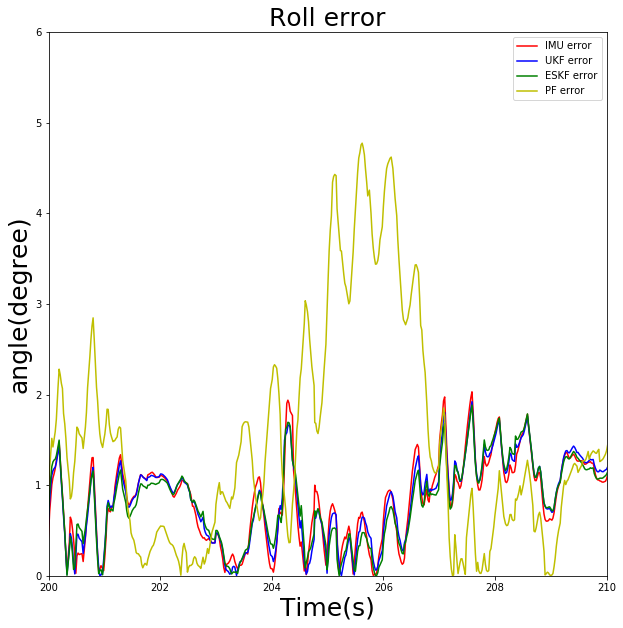
\includegraphics[width=0.7\textwidth]{figs/roll.png}
	\caption{Filter comparison - error in roll}
	\label{fig:ch:errorRoll}
\end{figure}

\begin{figure}[h]
\centering
	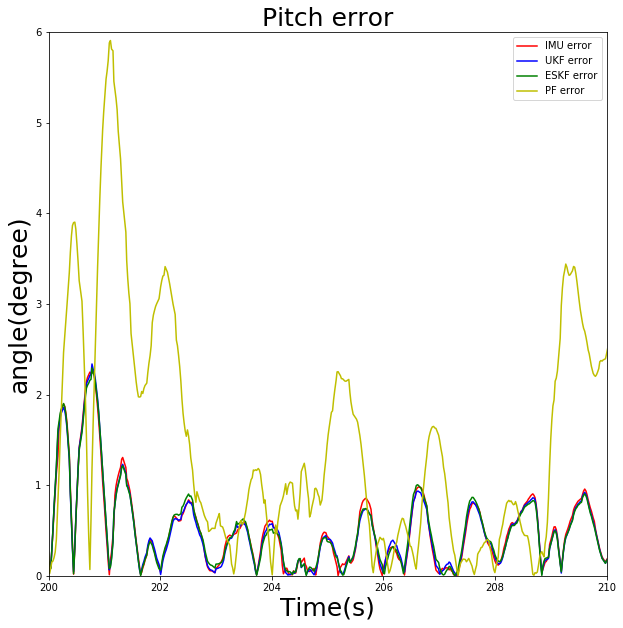
\includegraphics[width=0.7\textwidth]{figs/pitch.png}
	\caption{Filter comparison - error in pitch}
	\label{fig:ch:errorPitch}
\end{figure}

\begin{figure}[h]
\centering
	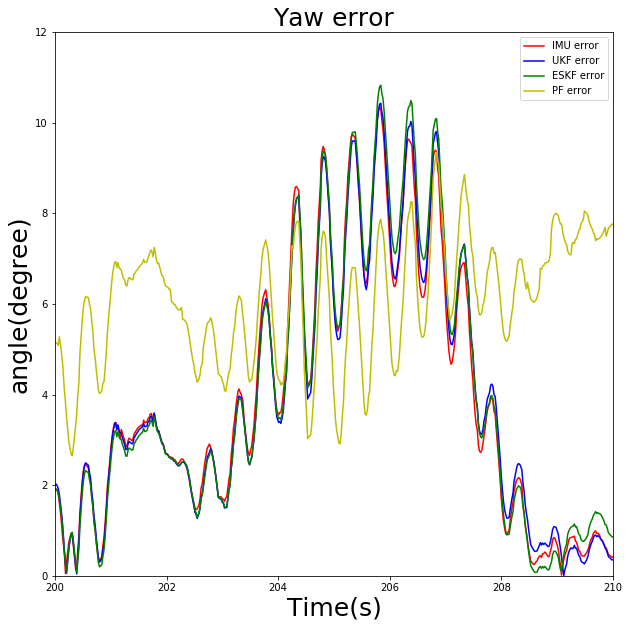
\includegraphics[width=0.7\textwidth]{figs/yaw.png}
	\caption{Filter comparison - error in yaw}
	\label{fig:ch:errorYaw}
\end{figure}


%%%%%%%% ch end %%%%%%%%%





%%%%%%%%%%%%%%%
\section{Sensor fusion mechanism}

Adding \gls{ZUPT} measurements has a significant effect on the accuracy of the yaw estimate, as seen from figure \ref{fig:pa:zuptYaw}. The yaw estimate error remains within the estimated error bounds (3$\sigma$ bounds), despite the fact that the magnetometer-estimated yaw is biased.

\begin{figure}[h]
	\centering
    \begin{subfigure}{\textwidth}
        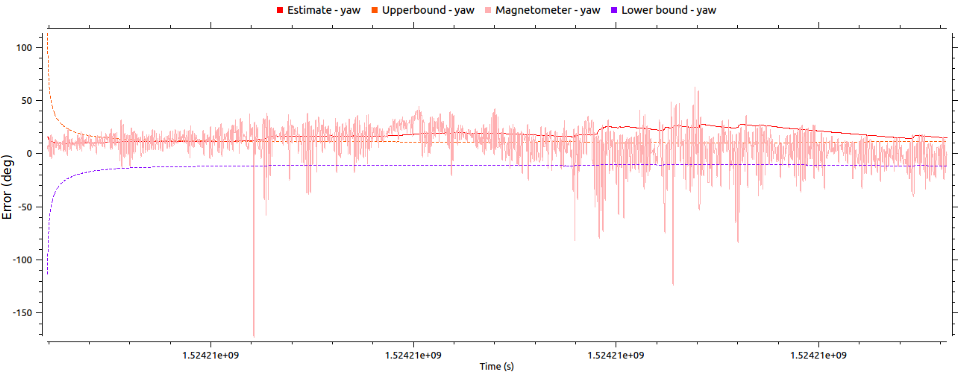
\includegraphics[width=\textwidth]{figs/yaw-without-zupt.png}
        \caption{Yaw estimate without \gls{ZUPT} measurements}
    \end{subfigure}
    \begin{subfigure}{\textwidth}
        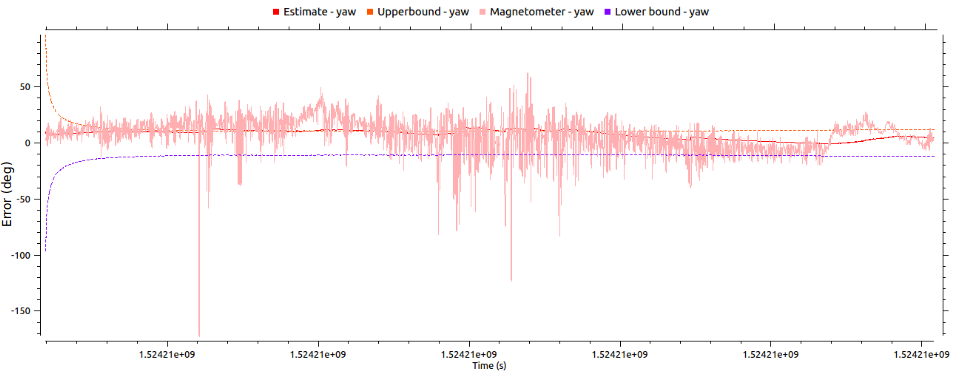
\includegraphics[width=\textwidth]{figs/yaw-with-zupt.png}
        \caption{Yaw estimate with \gls{ZUPT} measurements}
    \end{subfigure}
    \caption{Effect of \gls{ZUPT} measurements on the yaw estimate}
    \label{fig:pa:zuptYaw}
\end{figure}

